\documentclass{llncs}

\usepackage{pgf}
\usepackage{tikz}
\usepackage{xcolor}
\usepackage{graphicx}
\newcommand{\spazio}{\vskip 1.2ex}
\usepackage[english]{babel}
\usepackage[OT1]{fontenc}



\newcommand{\pp}{Decide-pp}


\newcommand{\treea}{

\begin{center}
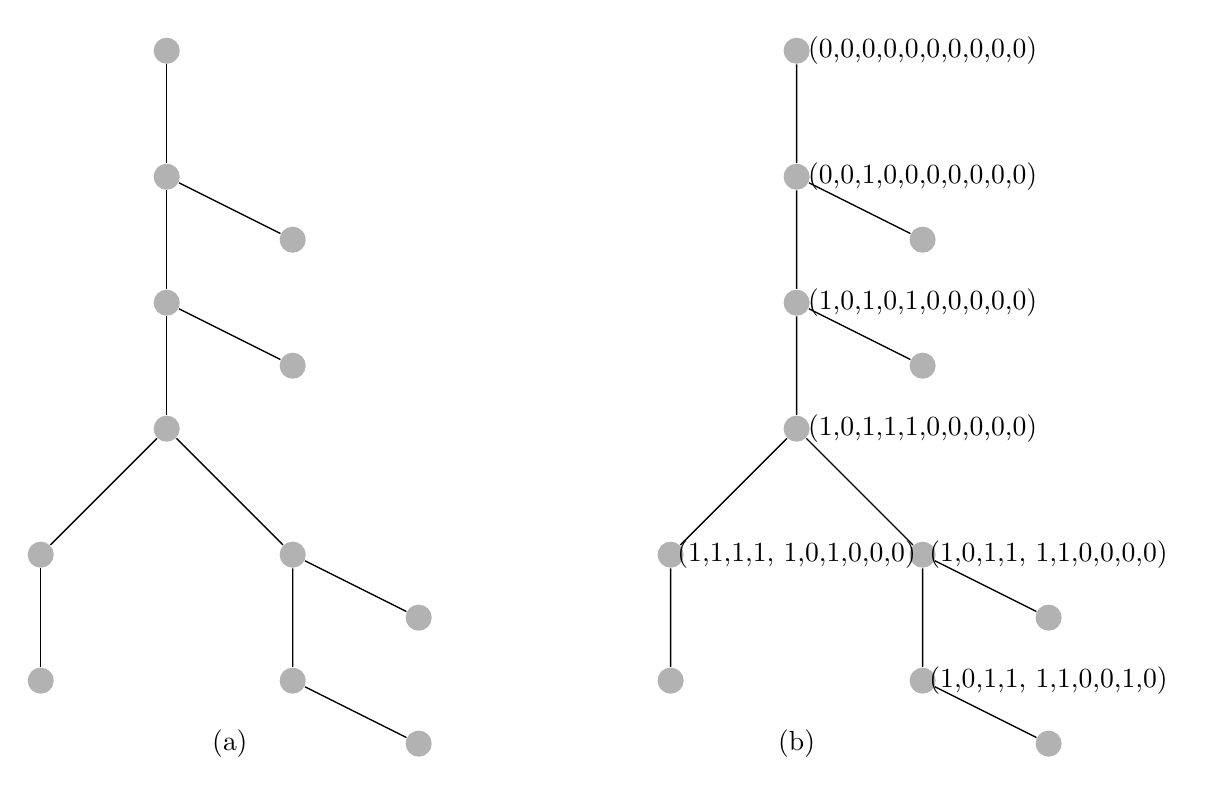
\begin{tikzpicture}[scale=0.8, line width=0.5pt,auto]
 \path
 (2,11)  node[circle,fill=black!30,minimum size=0.1cm](1)  { }
(2,9)  node[circle,fill=black!30,minimum size=0.1cm](2) { }
 (4,8)  node[circle,fill=black!30,minimum size=0.1cm](3) { }
 (2,7)  node[circle,fill=black!30,minimum size=0.1cm](4) { } 

(2,5)  node[circle,fill=black!30,minimum size=0.1cm](5) { } 
(4,6)  node[circle,fill=black!30,minimum size=0.1cm](4') { } 

(4,3)  node[circle,fill=black!30,minimum size=0.1cm](6) { }
(6,2)  node[circle,fill=black!30,minimum size=0.1cm](7) { }
(4,1)  node[circle,fill=black!30,minimum size=0.1cm](8) { }
(6,0)  node[circle,fill=black!30,minimum size=0.1cm](9) { }
(0,3)  node[circle,fill=black!30,minimum size=0.1cm](10) { }
(0,1)  node[circle,fill=black!30,minimum size=0.1cm](11) { };


\path[-,black] (1) edge[ ] node[left] {}  (2) ;
\path[-,black] (2) edge[] node[left]{} (3);
\path[-,black] (2) edge[] node[left]{}(4);
\path[-,black] (4) edge[] node[left]{}(5);
\path[-,black] (4) edge[] node[left]{}(4');
\path[-,black] (5) edge[] node[right]{}(6);
\path[-,black] (6) edge[] node[left] {} (7) ;
\path[-,black] (6) edge[] node[right] {} (8) ;

\path[-,black] (8) edge[] node[above] {} (9) ;
\path[-,black] (5) edge[] node[left] {} (10) ;
\path[-,black] (10) edge[] node[above] {} (11) ;



\path
 (12,11)  node[circle,fill=black!30,minimum size=0.1cm](1)  { }
(12,9)  node[circle,fill=black!30,minimum size=0.1cm](2) { }
 (14,8)  node[circle,fill=black!30,minimum size=0.1cm](3) { }
 (12,7)  node[circle,fill=black!30,minimum size=0.1cm](4) { } 

(12,5)  node[circle,fill=black!30,minimum size=0.1cm](5) { } 
(14,6)  node[circle,fill=black!30,minimum size=0.1cm](4') { } 

(14,3)  node[circle,fill=black!30,minimum size=0.1cm](6) { }
(16,2)  node[circle,fill=black!30,minimum size=0.1cm](7) { }
(14,1)  node[circle,fill=black!30,minimum size=0.1cm](8) {}
(16,0)  node[circle,fill=black!30,minimum size=0.1cm](9) { }
(10,3)  node[circle,fill=black!30,minimum size=0.1cm](10) { }
(10,1)  node[circle,fill=black!30,minimum size=0.1cm](11) { }


(3,0) node[](x){(a)}

(12,0) node[](x){(b)}

(14,11) node[](p){(0,0,0,0,0,0,0,0,0,0)}
(14, 9) node[ ](x) {(0,0,1,0,0,0,0,0,0,0)}
(14,7)  node[] (y) {(1,0,1,0,1,0,0,0,0,0)}
(14,5)  node[](z) {(1,0,1,1,1,0,0,0,0,0) } 
(16,3)  node[](v) {(1,0,1,1, 1,1,0,0,0,0) }
(16,1)  node[](m) {(1,0,1,1, 1,1,0,0,1,0)}
(12,3)  node[](n) {(1,1,1,1, 1,0,1,0,0,0) };


\path[-,black] (1) edge[ ] node[left] {}  (2) ;
\path[-,black] (2) edge[] node[left]{} (3);
\path[-,black] (2) edge[] node[left]{}(4);
\path[-,black] (4) edge[] node[left]{}(5);
\path[-,black] (4) edge[] node[left]{}(4');
\path[-,black] (5) edge[] node[right]{}(6);
\path[-,black] (6) edge[] node[left] {} (7) ;
\path[-,black] (6) edge[] node[right] {} (8) ;

\path[-,black] (8) edge[] node[above] {} (9) ;
\path[-,black] (5) edge[] node[left] {} (10) ;
\path[-,black] (10) edge[] node[above] {} (11) ;


\end{tikzpicture}
\end{center} }



 \newcommand{\forb}{
 \begin{center}
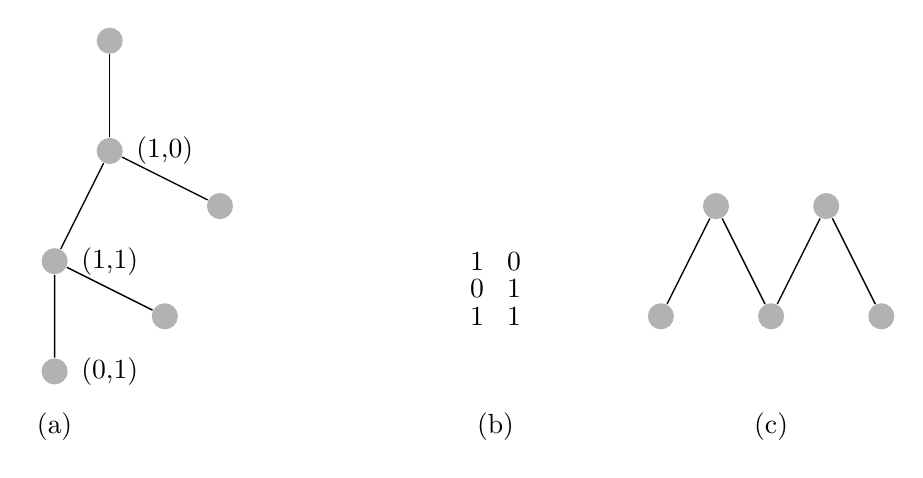
\begin{tikzpicture}[scale=0.7, line width=0.5pt,auto]
 \path
 (2,11)  node[circle,fill=black!30,minimum size=0.1cm](1)  { }
(2,9)  node[circle,fill=black!30,minimum size=0.1cm](2) { }
 (4,8)  node[circle,fill=black!30,minimum size=0.1cm](3) { }
 (1,7)  node[circle,fill=black!30,minimum size=0.1cm](4) { } 
(1,5)  node[circle,fill=black!30,minimum size=0.1cm](5) { } 
(3,6)  node[circle,fill=black!30,minimum size=0.1cm](6) { }

 (12,6)  node[circle,fill=black!30,minimum size=0.001cm](s1) { } 
(14,6)  node[circle,fill=black!30,minimum size=0.001cm](s3) {  } 
(16,6)  node[circle,fill=black!30,minimum size=0.001cm](s2) { }

 (13,8)  node[circle,fill=black!30,minimum size=0.001cm](a) { } 
(15,8)  node[circle,fill=black!30,minimum size=0.001cm](b) {  } 


 (1,4) node[](v){(a)}

(9,4) node[](u){(b)}

(14,4) node[](u){(c)}

(9, 7.5) node[ ](x) {\, \,  \, }
(9, 7) node[ ](x) { 1 \, 0}
(9,6.5)  node[] (y) { 0 \, 1}
(9,6.0)  node[](z) { 1 \, 1 }

(3,9)  node[](p){(1,0)}
 (2,7) node[](r){(1,1)}
(2,5)  node[](v){(0,1)};




\path[-,black] (1) edge[ ] node[left] {}  (2) ;
\path[-,black] (2) edge[] node[left]{} (3);
\path[-,black] (2) edge[] node[left]{}(4);
\path[-,black] (4) edge[] node[left]{}(5);
\path[-,black] (4) edge[] node[left]{}(6);
 

\path[-,black] (s1) edge[ ] node[ ] { }  (a) ;
\path[-,black] (s3) edge[ ] node[] { }  (a) ;
\path[-,black] (s3) edge[ ] node[ ] { }  (b) ;
\path[-,black] (s2) edge[ ] node[] { }  (b) ;


\end{tikzpicture} 
\end{center}
}




\newcommand{\graph}{
 \begin{center}
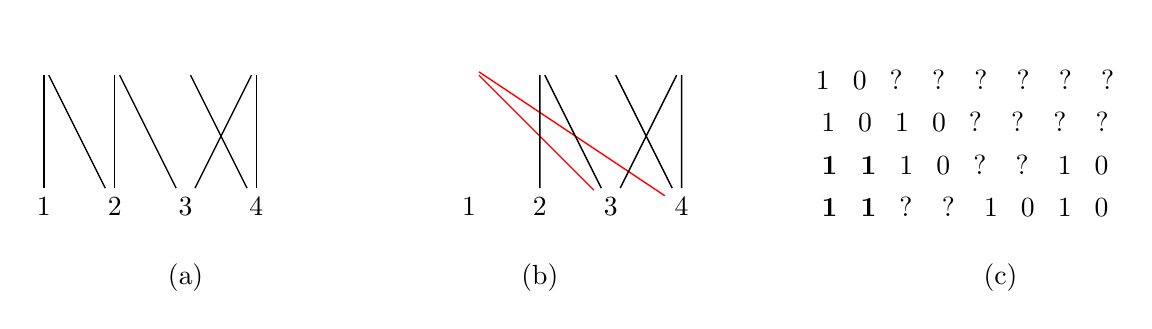
\begin{tikzpicture}[scale=0.9, line width=0.5pt,auto]
 \path
 (1, 5)  node[](a)  { }
(2, 5)  node[](b) { }
 (3,5)  node[](c) { }
 (4,5)  node[](d) { } 


(3,2) node[](x){(a)}

(8,2) node[](x){(b)}

(14.5,2) node[](x){(c)}


(14,5.40) node[] { \, \,     \,    \,     \,  \,    \,  }
 (14, 4.80)  node[] { 1 \,  0  \,   ?  \,   ?  \,   ? \,    ?  \,   ?  \,   ? }
    (14, 4.20) node [] { 1  \,   0  \,   1 \,     0   \,  ? \,    ? \,    ? \,    ? } (14,3.60) node [] { {\bf 1}  \,  {\bf 1} \,    1  \,    0 \,    ? \,    ? \,   1  \,   0} (14, 3.00) node [] { {\bf 1} \, {\bf 1} \,    ?  \,    ?  \,   1 \,   0 \,   1   \,  0} 



(1,3)  node[](1) {1} 
(2,3)  node[](2) {2} 

(3,3)  node[](3) {3}
(4,3)  node[](4) {4}

 (7, 5)  node[](a1)  { }
(8, 5)  node[](b1) { }
 (9,5)  node[](c1) { }
 (10,5)  node[](d1) { } 

(7,3)  node[](11) {1} 
(8,3)  node[](21) {2} 

(9,3)  node[](31) {3}
(10,3)  node[](41) {4};

\path[-,black] (1) edge[]  (a);
\path[-,black] (2) edge[]  (a);
\path[-,black] (2) edge[] (b);
\path[-,black] (3) edge[] (b);
\path[-,black] (3) edge[] (d);
\path[-,black] (4) edge[] (c);
\path[-,black] (4) edge[] (d) ;


\path[-,red] (31) edge[]  (a1);
\path[-,red] (41) edge[]  (a1);
\path[-,black] (21) edge[] (b1);
\path[-,black] (31) edge[] (b1);
\path[-,black] (31) edge[] (d1);
\path[-,black] (41) edge[] (c1);
\path[-,black] (41) edge[] (d1) ;

 



\end{tikzpicture}
\end{center}}



\newcommand{\grapho} {
 \begin{center}
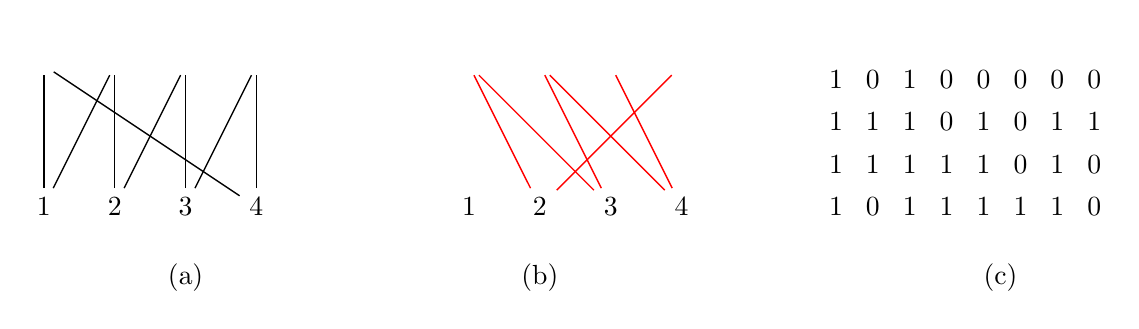
\begin{tikzpicture}[scale=0.9, line width=0.5pt,auto]
 \path
 (1, 5)  node[](a)  { }
(2, 5)  node[](b) { }
 (3,5)  node[](c) { }
 (4,5)  node[](d) { } 


(3,2) node[](x){(a)}

(8,2) node[](x){(b)}

(14.5,2) node[](x){(c)}


(14,5.40) node[] {   \,  \, \,   }
 (14, 4.80)  node[] { 1 \,  0  \,   1  \,   0  \,   0 \,    0  \,   0  \,   0 }
    (14, 4.20) node [] {1  \,   1  \,   1 \,     0   \,  1 \,    0 \,    1 \,    1 } (14,3.60) node []  {1 \,  1 \,    1 \,    1  \,    1 \,    0 \,   1  \,   0} (14, 3.00) node [] {  1 \,  0 \,    1 \,    1  \,   1 \,   1 \,   1   \,  0} 



(1,3)  node[](1) {1} 
(2,3)  node[](2) {2} 

(3,3)  node[](3) {3}
(4,3)  node[](4) {4}

 (7, 5)  node[](a1)  { }
(8, 5)  node[](b1) { }
 (9,5)  node[](c1) { }
 (10,5)  node[](d1) { } 

(7,3)  node[](11) {1} 
(8,3)  node[](21) {2} 

(9,3)  node[](31) {3}
(10,3)  node[](41) {4};

\path[-,black] (1) edge[]  (a);
\path[-,black] (2) edge[]  (c);
\path[-,black] (1) edge[]  (b);
\path[-,black] (2) edge[] (b);
\path[-,black] (3) edge[] (c);
\path[-,black] (3) edge[] (d);
\path[-,black] (4) edge[] (a);
\path[-,black] (4) edge[] (d) ;


\path[-,red] (21) edge[]  (d1);
\path[-,red] (21) edge[] (a1);
\path[-,red] (31) edge[] (b1);
\path[-,red] (31) edge[] (a1);
\path[-,red] (41) edge[] (b1);
\path[-,red] (41) edge[] (c1) ;



\end{tikzpicture}

\end{center}
}




\usepackage{graphicx}
\usepackage{amssymb}
\usepackage{amsmath}
\usepackage{epstopdf}
\usepackage{algorithmic}
\usepackage{a4wide}
\usepackage{verbatim}
\DeclareGraphicsRule{.tif}{png}{.png}{`convert #1 `dirname
#1`/`basename #1 .tif`.png}

\newcommand{\olds}[1]{\oldstylenums{#1}}
\newcommand{\oldsb}[1]{{\bfseries\olds{#1}}}
\newcommand{\mnote}[1]{\stepcounter{ncomm}\vbox to0pt{\vss\llap{\tiny\oldsb{\arabic{ncomm}}}\vskip6pt}\marginpar{\tiny\bf\raggedright {\oldsb{\arabic{ncomm}}}.\hskip0.5em#1}}
\newcounter{ncomm}






\newcommand{\grb}{ }
 \newcommand{\grbc}{, }
  \newcommand{\grbd}{. }
\newcommand{\g}{}
\newcommand{\m}{}
\newcommand{\md}{ }
\newcommand{\bset}{}
\newcommand{\mdim}{}
\newcommand{\me}{{} }
\newcommand{\mec}{{}, }
\newcommand{\med}{{}. }
\newcommand{\sfree}{-free }
\newcommand{\card}[1]{}
\begin{document}
\title{The Binary Perfect Phylogeny with Persistent Characters}
\author{Paola Bonizzoni\inst{1} \and Chiara Braghin \inst{2} \and Riccardo Dondi\inst{3} \and Gabriella Trucco \inst{2}
}

\institute{Dipartimento di Informatica Sistemistica e Comunicazione \\
Univ.  degli Studi di Milano - Bicocca \\
Viale Sarca 336, 20126 Milano - Italy \\
\email{bonizzoni@disco.unimib.it}
\and
 Dipartimento di Tecnologie dell'Informazione
Univ. degli Studi di Milano, Crema \\
\email{chiara.braghin@unimi.it;gabriella.trucco@unimi.it}
\and 
Dipartimento di Scienze dei Linguaggi, della Comunicazione e degli Studi Culturali \\
Univ. degli Studi di Bergamo, Bergamo  \\
\email{riccardo.dondi@unibg.it}.
\email{}}

\pagestyle{plain}
\date{march}\maketitle



\begin{abstract}
The  binary perfect phylogeny model is too restrictive to model  biological events such as back mutations. In this paper we consider a  natural generalization of the  model that allows a special type of back mutation.  We investigate the  problem of reconstructing  a  near perfect phylogeny over a binary set of characters where   characters are {\em persistent}:
 characters  can be  gained and lost at most once. Based on this notion, we define the problem of  the Persistent Perfect Phylogeny (referred as P-PP). 
We restate the P-PP problem  as a special case of the Incomplete Directed Perfect Phylogeny,  called Incomplete  Perfect Phylogeny with Persistent Completion, (refereed as IP-PP),  where the instance is an incomplete binary matrix   having some missing entries, denoted by symbol , that must be determined (or completed) as  or  so that   admits a binary perfect phylogeny.
We show that the IP-PP problem can be reduced to a problem over an edge colored graph since the  completion of  each column of the input  matrix  can be  represented by a graph operation. 
  Based on this graph formulation,  we develop  an exact algorithm  for solving  the P-PP problem that is exponential in the number of characters and polynomial in the number of species. 
\end{abstract}


\section{Introduction}



The perfect phylogeny   is one of the most investigated models  in different areas of computational biology.
This model derives from a restriction of the parsimony methods  used to reconstruct the evolution of species (taxa).
Such methods assume that each taxon is characterized by a set of of attributes, called characters. In this paper we focus on the binary perfect phylogeny model; characters can take only the values (or states) zero or one, usually interpreted as the presence or absence of the attribute in the taxa.  Restrictions on the type of  changes from zero to one and vice versa lead to a variety of specific models  (Felsenstein, \cite{Fel}). In the  Dollo parsimony, a character may change state from zero to one only once, but from one to zero multiple times  \cite{Pr1}.  In the variant of Camin-Sokal parsimony \cite{CS},  characters are {\em directed}, only changes from zero to one are admissible on any path from the root to a leaf. This fact means that  the root is assumed to be labeled by the ancestral state with all zero values  for each character, and  no character change back to 0 is allowed. This last variant is  known as the binary directed perfect phylogeny, and it has  a linear time solution \cite{Gus91}. 

Such a  model has been successfully applied  in the context of haplotype inference, starting from the seminal work by Gusfield on the   Perfect Phylogeny Haplotyping Problem \cite{Gus02}.  This last problem has been widely investigated, and very efficient polynomial time solutions have been proposed, including   linear-time algorithms \cite{Gus06}, \cite{Mu}, \cite{Boniz}. However, the real data usually do not fit the simple model of the binary perfect phylogeny and thus in the past years generalizations of the model have been proposed.  Some models are surveyed in \cite{FB00}.


A central goal in this investigation  of the binary perfect phylogeny model is to extend its applicability by taking into account the biological complexity of  data, while retaining  the computational efficiency where possible. More precisely, the binary perfect phylogeny model though allowing a very efficient reconstruction is quite restrictive to explain the evolution of data where   homoplasy events such as back mutations, also called reversals,  are present.  In order to include such events,   the problem of reconstructing the near-perfect phylogeny    has been formalized and investigated.  Some work has been done to produce algorithmic  solutions to the problem, mainly fixed-parameter algorithms have been provided \cite{near-perfect2}, \cite{near-perfect1}.
However,  the near-perfect phylogeny   model appears to be too general for some biological applications.  The model  does not distinguish the main two types of homoplasy occurring in a phylogenetic tree: recurrent mutation  and back mutations.    Back mutations are changes in the  state of the character that only occur along the same path from the root of the tree. On the contrary,  recurrent mutations are changes  in the  state of  the  character  that occur  along different paths of the tree, since the character is allowed to label multiple edges of the tree. In this paper we address the problem of constructing a perfect-phylogeny under the assumption that  only a special type of back mutation  may occur in the tree. A character may change state only twice in the tree,  precisely from  to  and from  to ,  and the changes occur along the same path from the root of the tree . These characters have  already been considered in the literature  and called {\em persistent}  by T. Przytycka \cite{Pr06} in a general framework of tree inference.  More precisely,  in  \cite{Pr06},  the change of a character from state  to  models the gain of  the character, while the change from  to  models the loss of the character.  
The use of the notion of persistent character is quite relevant when reconstructing phylogenies that describe the gain and loss of genomic characters \cite{zeng}.  An example of a promising class of genomic characters (also called rare genomic changes - RGC - ) is given by  insertion and deletion  of ‘‘introns’’ in protein-coding genes during the evolution of eukaryotes. In this framework,   persistent characters allow to infer phylogenies by using the gain and loss of introns \cite{zeng}. 

We define a generalization of the (rooted) binary directed perfect phylogeny  where each character may be persistent.   Clearly our model is a restriction of the Dollo parsimony,  where characters can be lost several times, i.e. a character can be lost along different paths from a root to a leaf. Acquisition or loss of characters (i.e. attributes) when
unrestricted could make  the reconstruction of an  evolutionary tree difficult, if not possible.





 Assume that  is a
set of {\em species} and  is a set of
{\em characters}. In the paper we consider binary matrices representing
species and characters. More precisely,    a binary matrix
 of size  has columns associated with the set
 of characters, i.e. column  represents character , while rows of  are associated with the set  of
species, i.e. row  represents species . Then 
if and only if species  has character , otherwise . 

In the rest of the paper,  to simplify the notation, we identify rows with species and columns with characters.


The gain of a character in a  phylogenetic tree is usually represented by an edge labeled by the character.   In order to  model  the presence of persistent
characters, the loss of a
character   in the tree is represented  by  an edge that  is labeled by the negation of , or negated character, denoted by  .   Clearly, an edge labeled by a negated character  follows  an edge labeled by the  character along a path from the root to a leaf.  
 The following definition is based on the  general  coalescent model given in \cite{EHK} to  represent the evolution of    haplotype sequences and assume that nodes are labeled by vector states of characters.



Formally, we have:

{\bf Persistent Perfect Phylogeny}
Let   be a binary matrix of size . Then a {\it
persistent perfect phylogeny}, in short  {\em  p-pp tree} for , is a rooted tree 
that satisfies the following properties:

\begin{enumerate}

\item each node  of  is labeled by a vector  of length ;

\item  the root of  is label  by a vector of all zeros,  while  for each  node  of  
the value  represents  the state,   or  respectively, of character  in tree ;

\item   for each character  there are at most  two  edges  and  
such that  and  
(representing a change in the state of ) such that ,   occur along the same path 
from the root of  to a leaf of ; if  is closer to the root than , then 
 the  edge  where  changes from  to  is labeled , 
while  edge  is labeled ,

\item  each row  of   labels exactly one leaf of .

\end{enumerate}

In the classical  definition of a  Perfect Phylogeny Tree,  in short {\em pp} tree, 
no negated characters are allowed in the tree (see \cite{Setubal}) (see definition in Section \ref{pre1}). Observe that by the above definition  of p-pp tree,  for each  leaf  of tree , the positive characters that label edges 
that are along the unique path from the root to  and
do not occur as  negated along the same path, specify  exactly the characters
that have value  in the row     of .

Thus, let us state the main problem investigated in the paper.

\noindent

{The \bf  Persistent Perfect Phylogeny
 problem (P-PP):} Given a binary matrix ,  returns a p-pp tree for  if such a tree exists.
 

 
 \vspace{.2in}
 
 In the paper we investigate the  solution of the P-PP problem. Our main contribution is a graph-based restatement of the problem that allows us to provide an exact algorithm for the problem having a worst time complexity that is polynomial in the number   of rows of the matrix and exponential   in the number  of characters.  
Since in  real data the number of characters is usually small, while the number of species may be very large, the algorithm could be  efficient even on large instances  as shown by an experimental analysis illustrated in Section \ref{experiment}.
 


 The graph-based solution of   the P-PP problem is obtained by  restating the problem as a  variant of the Incomplete Directed Perfect Phylogeny \cite{Sha}, called Incomplete  Perfect Phylogeny with Persistent Completion (IP-PP), where the input data of this last problem is a specific incomplete matrix   over values   and the goal is to complete values  into  or  so that  admits a classical perfect phylogenetic tree.
Then we show  that the IP-PP problem reduces to the problem of reducing a colored graph by a graph operation  that represents  a completion of a column of the input matrix.    Based on these ideas we discuss our exact algorithm for the P-PP problem.
 
  We believe that the graph-based formulation of the problem could help in investigating polynomial time solutions to the problem. 

 

 
 \section{The Perfect Phylogeny model: preliminaries}
 
 \label{pre1}
 
  
Let us give the definition  of a perfect phylogeny for a binary matrix  and  some relevant basic results that will be used in the paper.
 
 
 \noindent
 {\bf Perfect Phylogeny}
 
 Let   be a binary matrix of size . Then a {\it directed
perfect phylogeny}, in short  {\em  pp tree} for , is a rooted tree 
that satisfies the following properties:

\begin{enumerate}
 
 \item each node  of  is labeled by a vector  of length ;
 
 \item  the root is labeled  by a vector of zeros, while for each  node , the value 
  represents  the state,   or  respectively, of character  in tree ;

\item  for each character  there is at most one edge , labeled , such that
 (notice that , while );
edge  represents a changing of state of ; 

\item each row of matrix  labels exactly one leaf of .

\end{enumerate}
 
The algorithmic solution of the Perfect Phylogeny model has been investigated in \cite{Gus91}, where a linear time algorithm is provided. 
In particular, the paper \cite{Gus91} provides a well known characterization of matrices admitting a perfect phylogeny.
A binary matrix  admits a perfect phylogeny if and only if it does not contain a pair of columns and three rows inducing    the configurations  and ,  also known as   {\em forbidden matrix} (see Figure \ref{forb} (b)). We will use this  characterization  in the paper.

In particular, the forbidden matrix has a representation by means of a  graph consisting of a path of length four containing three species and two characters; this graph  is   called -graph. Such a graph is obtained by drawing an edge between every pair of  species and  characters having value  in the matrix (see Figure \ref{forb} (c)). 

Notice that the forbidden matrix is the smallest matrix that does not admit a pp tree. However, by allowing a character to be persistent, the matrix admits a persistent perfect phylogeny, as shown in Figure \ref{forb} (a).

A well known concept that  has been used several times in the framework of the perfect phylogeny is a graph representation of the four configurations , ,  and  (called four gametes): the {\em  conflict graph}. 
We say that two positive characters  of matrix  are in {\em conflict} in matrix  , if and only if   the pair of columns  of  induces the four gametes.





\begin{definition}[conflict graph]
\label{sigmag}
Let  be a binary matrix.
The {\it conflict graph} associated with  matrix  is the
undirected graph  where  a pair  if and only if  are in conflict in matrix  .
 \end{definition}



Notice that when   has  a  conflict graph with no edges,    does not necessarily admit   a rooted perfect phylogeny,  since  could contain an occurrence of the forbidden matrix. For example, the forbidden matrix has a conflict-graph with  no edges.

In this paper we define a variant  of the the Incomplete Directed Perfect Phylogeny (in short IDP)   \cite{Sha}. The input data of the IPP problem is a matrix over symbols  where symbol  is used to denote  an entry of the matrix that is not determined. Then the IPP problem is finding a completion of the matrix, i.e. assigning values  to  symbols so that the matrix admits a perfect phylogeny.   

For basic  notions of graph theory used in the paper see \cite{Cormen}.



\begin{figure}[ptb]
\begin{center}
\forb

\end{center}
\caption{The Figure (a) illustrates the perfect persistent phylogeny for the forbidden matrix reported in Figure (b) and the -graph for the forbidden matrix in Figure (c). 
} 
\label{forb}
\end{figure}
 
\section{The Incomplete  Perfect Phylogeny with Persistent Completion}


Let  be a binary  matrix which is an
instance of the P-PP problem. The  {\em extended matrix} associated with  is a matrix \me of size \ over alphabet   which is obtained by replacing each column  of  by a pair of columns , where  is the positive character, while  is the negated character,  moreover for each   row   of , it holds:


\begin{enumerate}
 

\item    if , then   and ,

\item    if , then   and .
\end{enumerate}






Informally, the assignment of the pair  in a species row  for the pair of   entries in columns  and  means that character  could be persistent in species , i.e. it is gained and then lost. On the contrary, by definition of a persistent perfect phylogeny,  the pair  assigned in  a species  row  for the pair of   entries in columns  and , means that character  is only gained by the species .

In the paper, we will use  the term extended matrix to denote an extended matrix associated with a binary matrix and defined as above. 
A {\em completion  of  a character }   of matrix \me  is
 obtained by solving the pair  given in  the pair of columns   , 
     by the   value  or
.   If a character   is completed,  then it is  called {\em active}. 


A  {\em completion  of matrix}   \me is a completion
of all characters of \mec while a {\em partial completion  of} \me
is a completion of zero  or more  characters of \med


Figure \ref{me} (a) shows an example of  input  matrix  for the P-PP problem. Then Figure \ref{me} (b) shows the incomplete  matrix \me associated with . A possible completion of \me is given in  Figure \ref{me} (c). 



\begin{figure}[htbp]
\begin{center}
\begin{tabular}{c c c c c  c c c c c c c c c c   c c c c c c c c c c  c c c c c c c c c c   c c c c c c c c c c}

 &  &  &  &  & & & & & & & & & & & &  & &  & &  & &  & & & & & & & & & & & & &  &  &  &  & &  &  & &  & \\
0 & 0 & 1 & 1 & 0 & & & & & & & & & & & ?&  ?&  ?&  ?& 1&  0& 1&  0& ?&  ?& & & & & & & & & & & 1& 1&  1& 1&  1&  0& 1&  0& 0&  0\\
0 & 1 & 0 & 0 & 0 & & & & & & & & & & & ?&  ?&  1&  0& ?&  ?& ?&  ?& ?&  ?& & & & & & & & & & & 0& 0&  1& 0&  0&  0& 0&  0& 0&  0\\
1 & 0 & 0 & 0 & 0 & & & & & & & & & & & 1&  0&  ?&  ?& ?&  ?& ?&  ?& ?&  ?& & & & & & & & & & & 1& 0&  1& 1&  1&  1& 0&  0& 0&  0\\
1 & 0 & 0 & 0 & 1 & & & & & & & & & & & 1&  0&  ?&  ?& ?&  ?& ?&  ?& 1&  0& & & & & & & & & & & 1& 0&  1& 1&  1&  1& 0&  0& 1&  0\\
1 & 1 & 1 & 0 & 0 & & & & & & & & & & & 1&  0&  1&  0& 1&  0& ?&  ?& ?&  ?& & & & & & & & & & & 1& 0&  1& 0&  1&  0& 0&  0& 0&  0\\

\multicolumn{5}{c}{(a)} & & & & & & & & & & & \multicolumn{10}{c}{(b)}  & & & & & & & & & & & \multicolumn{10}{c}{(c)}\\


\end{tabular}
\end{center}
\caption{The figure  illustrates a binary matrix \m (a) and its  extended matrix \me (b)  and a completion of \me  (c).}
\label{me}
\end{figure}


We introduce below a problem to which we reduce P-PP, as shown in Theorem \ref{equivalence}.



\noindent
{\bf Incomplete  Perfect Phylogeny with Persistent Completion  Problem (IP-PP)}

{\em Instance:} An extended matrix   over   .  

{\em Question:}  give a  completion  of the extended   matrix    such  that  admits a perfect phylogeny, if it exists.

\vspace{.2in}

Thus we state the first result of the paper. In order to prove the result we assume that the input matrix   does not have columns consisting of zeros, that is for each character , there must exist a species having the character. As a consequence of this assumption, given the extended matrix  of , it must be that for each positive character  there is a species having   the positive character   and not the negated character .

\begin{theorem}
\label{equivalence}
Let   be a binary matrix and  the extended matrix   associated with . Then   admits a p-pp tree if and only if there
exists a  completion  of    admitting
a pp tree.
\end{theorem}
\begin{proof}
({\em If }) Let  be  a  completion of matrix  such that  admits a  perfect phylogeny  .


In the following we show that apart from the labeling of internal nodes of tree , the tree  is a p-pp  tree for matrix . More precisely, we obtain  a  p-pp tree  for matrix  by changing the labeling of tree  as follows. 
In order to distinguish the labeling of node  in tree  from the new labeling of the same node  in tree , we denote the new labeling of  in  by the vector .
Given 
a node  of tree  labeled by a  vector , then the label    of node  in tree   is defined as follows:

for each , with ,  if and only if  and , otherwise  
Informally, a character  has value  in vector  if and only if   occurs as   in vector  and it is does not occur as negated in , that is  character  has value  in .

We first show that property (4) of the definition of a persistent perfect phylogeny holds for tree  for matrix , i.e. each row  of  labels a leaf  in tree . Now, row  of the completion  labels a leaf   of tree .
We can easily show that  is equal to row  in matrix .   
This fact follows from the observation that characters that have value  in row  of  still have value  in row  of the completion . By definition of a completion, only   a character having value  in  may be persistent
along a path of tree , i.e. it labels  an  edge of the path and its negated character labels another edge of the same path.
Consequently, the characters associated with the edges along the unique path of  from the root to  and which are not negated are exactly those having value  in row  of , that is  is equal to row  of , as required.


Now,   properties (1) to (3)  given by definition of a persistent perfect phylogeny  for matrix  follow from the fact that  is a perfect phylogeny for matrix , and thus each character is associated with exactly one edge of the tree, which implies the same property for each negated character .  Observe that by  definition of extended matrix a negated character occurs in a row if and only if its positive character occurs in the same row.  Moreover, since we assume that  for each character  matrix  must have a a species that contains  the positive character , but not the negated character , 
 it is immediate to verify that every negated character  follows character  along a path from the root to a leaf, thus proving that change of state of  from  to  (that is from  to  in tree )  occurs after the change of state from  to  of character .  In fact, by definition of a completion the set of species  having character  includes the set of species having character , since columns  and  both have values  or  has value  and  has value .

 


({\em Only if }) Vice versa, let us now show that if there exists a persistent perfect phylogeny  for matrix , then there exists a completion  of  such that  admits a perfect phylogeny.
We can associate to tree  a matrix  of size  as follows.
  For each  character  of  add a new column . Then consider each row  of matrix  such that
   a negated character  occurs along the path from the root to . Then set  value  for row    in columns   and  of matrix .
Notice that   is a completion of  and clearly  is a perfect phylogeny for . 
\qed
\end{proof}






\section{The red-black graph}
\label{section-graph}

 
In this section  we give a graph representation of  an extended matrix, and we define a graph operation that represents  a special type of completion of  the pair of  columns of the matrix associated with a  character.  


Let  be an extended matrix , then  the {\em red-black} graph  for matrix  consists of the edge colored graph  where ,  given  and  the set of positive characters and species of matrix , while  is defined as follows:
 is a black edge  if and only if  and .




 




Then we define a graph operation  on nodes (characters) of the graph \grb that represents a {\em canonical} completion of characters  and consists of adding red edges, removing black or red edges. 
This  graph  operation  over characters (nodes)  of  the red-black graph may be iterated till the graph has only {\em active} characters, as defined below.




\noindent
{\bf Realization of a character   and its canonical completion}

Let    be the connected component of graph \grb containing node .  The {\it realization of   character }  in graph \grb  consists of:

\begin{itemize}



 \item  (a) adding  red edges connecting character  to all species nodes  that are in  and such that  is not an edge of \grbc
  
   \item

  (b) removing  all black edges  in graph \grbc  Then  is labeled {\em active}.
  
  \item (c) if  a character  is connected by red edges to all species of ,  then   is called  {\em free}.  Then its outgoing edges are deleted from the graph.  
 
 \end{itemize}
 
 The realization of a character  is associated with a special  completion in matrix  of the given character, called canonical.
The {\em canonical} completion of  character  in matrix  is defined by completing
each pair   occurring in the pair of  columns  and  as follows:
the pair   is completed by    in  every species  that is in the  component  of graph \grbc while value    is assigned in the remaining  rows.




\begin{figure}[ptb]



\graph
\caption{The Figure (a) illustrates the  graph \grb of the extended matrix associated with the matrix   of  Example \ref{ex}.  Then  (b)   illustrates the graph  \grb after the realization of character .  Then (c)  illustrates \me after the completion of .}
\label{graph4x4}
\end{figure}



 \begin{example}
 \label{ex}
Figure \ref{graph4x4} (a) illustrates   the red-black graph  of the  extended matrix  associated with matrix  consisting  of rows  , numbered   and , respectively.  Characters of  are denoted by letters  and . Then Figure \ref{graph4x4} (b) illustrates  the red-black graph obtained     after the realization of   character , while Figure \ref{graph4x4} (c) reports  the corresponding canonical completion in \me of character .


\end{example}



Informally, the red edges of graph \grb  incident to a character  that has been realized  represent  the  pairs   in columns     that are completed as  in matrix . 

In the following we call  {\em e-empty} a red-black graph without edges.

\begin{remark}
\label{remark-sigma}

Let  be a sequence of  all characters of a red-black graph for an extended matrix , and let    be the graph produced after the realization of the characters in  one after another.  Clearly,  the realization of characters in  produces a completion of the matrix .  Then, either  is e-empty or  contains two nodes inducing a   -graph. Observe that if   is not e-empty, it must have only red edges  that are  incident to at least two characters of the graph.   In fact,  assume on  the contrary that  has a single character   that  is incident to red edges. Then  must be connected  to all species nodes in the same connected component of the graph. But, this fact leads to a contradiction  since   is free and all red edges incident to  are deleted from the graph. By  inspection of the possible cases, it is easy to verify that the   minimum size connected component of  induces a -graph consisting of two characters and three species. 
 Such a graph represents the presence of a  forbidden matrix in the  completion  of matrix ,  and  hence  does not admit a  perfect phylogeny (see Section \ref{pre1}). 


\end{remark}

The following example illustrates an application of the previous Remark \ref{remark-sigma}.


\begin{example}
\label{exx}
Let   be  a matrix  having the four characters , ,  and  and rows , ,  and , numbered  and , respectively.   Let   be the graph obtained after the realization of the sequence   of characters.  Then  consists  of  the path  with red edges. Then graph  induces the -graph consisting of path  .   Observe that the completion  of  the extended matrix  of  consists of rows , ,   and  and such a matrix does not admit a perfect phylogeny as characters  and  and species  induce the forbidden matrix in the completion .
Figure \ref{grapho} illustrates the example.
\end{example}

\begin{figure}[ptb]



\grapho
\caption{The Figure (a) illustrates the  red-black graph of the Example  \ref{exx} .  Then  (b)   illustrates graph  of the example,  while (c)  illustrates   the completion of  induced by the realization of sequence .}
\label{grapho}
\end{figure}


Since
 we are interested in computing  canonical completions of the matrix that admit a pp tree   by  the previous Remark \ref{remark-sigma} only canonical completions that are obtained by the realization of  special   sequences of characters of the red-black graph are considered, as defined below.

\begin{definition}

\label{suc-red}
 Given a graph \grb for an extended matrix \mec  a {\em successful  reduction} of \grb is an ordering   of  the set of positive  characters  of the matrix such that the 
consecutive realization of each character in  (which removes
 black edges from graph )   leaves an   e-empty red-black graph.

\end{definition}

In   Section \ref{prova}, we show that finding a solution to an instance  of the IP-PP problem   is equivalent to computing the existence of a successful reduction for the red-black graph for the input matrix.
More precisely, let  be an instance of the IP-PP problem.  In the following Theorem   \ref{main-reduction},  we prove  that if   \me admits a pp tree , then there exists a successful reduction of graph .
Vice-versa,  we show that  a successful reduction of  the red-black graph for   provides a completion  of the matrix \me that admits a pp tree, thus giving   a  solution to the IP-PP instance..  



\begin{theorem} \label{main-reduction}   Let \me\ be an extended matrix.
Then  \me\ admits a   perfect phylogeny,  if and only if
 there exists a successful reduction of the graph \grb \ for \med

\end{theorem}

\subsection{Building   a successful reduction from a pp tree}

\label{prova}

This section is devoted to the  proof of  one direction of  Theorem  \ref{main-reduction}, that is showing  how to get a successful reduction from a pp tree.    We  will use the following remark that holds for extended matrices.




In this section, given a node  of tree , by  we denote the subtree of  having root . Moreover, we assume that edges of a tree  are oriented. The orientation of edges is  from the root to a leaf node. 









\begin{remark}
\label{annotated0}
Let  be a pp tree for a completion of an extended matrix . Then by definition of a perfect phylogeny is immediate to verify that the root  of tree      is  a  binary vector of size , moreover each internal  node   is labeled by a -vector  defined as follows: each entry  has value  if and only if the  corresponding th  character (positive or negated) occurs along the path from the root of the tree  to node .

\end{remark}


\begin{example}
\label{ex2}

Figure \ref{treea} (a)  illustrates  the pp tree for matrix  of Figure \ref{me} (c). Notice that rows of matrix  are numbers , while the positive characters are . Then Figure \ref{treea} (b) illustrates the vectors  labeling each internal node  of  tree . 


\end{example}

\begin{figure}

\begin{center}
\treea
\end{center}
\caption{The Figure (a) illustrates a perfect persistent phylogeny  for the matrix of Example \ref{ex2}. Figure (b) reports the vector  for each node  of the tree .}
\label{treea}
\end{figure}



Then  we need to state some technical lemmas and introduce a normal form for a pp tree, called {\em standard}. A tree   is in {\em standard form} when it is in {\em simple form} as defined below and satisfies the properties stated in Definition \ref{standard}.

A pp tree   is in  {\em simple form } if and only if  each edge of the tree is exactly labeled by one character and  does not contain  two  edges  incident to the same node,  one labeled by character  and the other labeled by , respectively.  

Given  a pp tree for a completion , we can show that tree  can be reduced to one in simple form. This fact implies that we can obtain from    a  completion   that admits a tree in simple form. Then the completion   is called {\em simple completion}.

\begin{lemma}
\label{tec0}
If  has a completion that  admits a pp tree, then  there exists a simple completion  of .  
\end{lemma}

\begin{proof}
Let  be the pp tree  for a completion of  and 
assume that  is not in simple form.  We first transform the tree  into a tree  such that each edge has only one label. Tree  is   obtained by replacing each edge   with  labels with a path of  edges each one labeled with a distinct label of the replaced edge . On the contrary, an edge without labels is contracted, in the sense that the two end nodes of the edge are collapsed to a unique node. Clearly, the above two operations do not change the completion  .



Assume now that there exists two edges  in  tree  that are incident to the same node and are labeled by  characters  and , respectively. Assume that  and .  

Then we can move tree  as a subtree of  node  by removing edge   and making the root  adjacent with node . Then change the completion  by replacing all pairs  induced by the columns  and   and species row in subtree ,  by the pair , obtaining the completion . It is easy to verify that  is the tree representation of the completion .
We can iterate the above operation and obtain a tree in standard form, as required by the lemma.
\qed


\end{proof}

Let  be the red-black graph for an extended matrix   and let   be   the pp tree of a completion of .

We require that  a  tree  that is in simple form  satisfies  an additional property  that relates the tree  to the red-black graph  .  Observe that we associate to each node  of  the red-black graph that is obtained by the realization of the positive characters that have value  in vector  where if  a negated character  is free, then its incident red edges are removed from the graph  if and only if    has value  in vector . We define such a graph, denoted as , the {\em red-black graph for node } of .




\begin{definition} [standard property]
\label{standard}
Let  be a pp tree  in simple form for a completion . Then  is in standard form if and only if the following property holds:
for each node    of  such that  is an edge of the tree  labeled   or ,    all species of tree  are the same species that are in the  connected component of  graph  containing node .

\end{definition}



\begin{lemma}
\label{tec1}
Let   be an extended matrix admitting a pp tree. Then, matrix  admits a completion that is represented by a tree  in standard form.
\end{lemma}

\begin{proof}
By Lemma  \ref{tec0} we can assume that the matrix  has a simple completion  
that is represented by a tree  in simple form.
To prove the existence of a tree  in standard form, we iterate the application of the following procedure to  till it is in standard form.  Each iteration of the procedure corresponds to changes to the completion ,
such that the  final computed completion   is represented by the new tree in standard form. 
Let  be the node that is closest to the root  of , such that  does not satisfy  the property stated in Definition \ref{standard}.  Eventually,  may be the root of .
 Let  be the connected component of  the red-black graph   having node .  Since property of   Definition \ref{standard} is violated then the following two cases are possible.
Case 1: there exists a species  in component  and  is not in subtree .
Case 2:  there exists a set  of species in the subtree  that are not in .


In the following we show that Case 1 leads to a contradiction, while in Case 2 we built  from tree   a new pp tree  for a completion of matrix   where node  does not verify Case 2 and thus  must satisfy Definition \ref{standard}.


 {\em Case 1.}
 
Assume that there exists a species in component  that is  not in subtree .
In the following we show that we obtain a contradiction.  If Case 1 holds, then there must exist a species   that is not in tree   and  is connected in component  (by  red or black edges) to a species  of tree   by means of character . More precisely, in component   is connected to characters   and , while  is connected to character .  Since  is not in tree , species  and  must have a common ancestor that is a node  along the path  from the root  to node .    
Then  character  labels an edge that occur on path  and thus  occurs before node .  Consequently,    is realized in graph , thus implying that  is connected  only by red edges to species  and . This fact implies that both   do not have character  and thus it holds that   labels an edge that occurs along the path from the root of  to the common ancestor node  of  and . 
 Since Definition \ref{standard} holds for each node that precedes ,  it follows that all species in  are in a connected component  that contains , where  is connected to all species in  by red edges. Consequently,   is free in  and thus all red edges connecting  to  are removed from the red-black graph , by definition of red-black graph associated to a node, a contradiction
with the previous assumption. It follows that  species  cannot be in component , thus implying that no other species different from the ones in   can be in component .
 
 {\em Case 2.}
 
 Assume that  is the largest set of species that are in  and are not in the component 
. 
By definition of pp tree, it must be that the set of species  is in the subtree  for a node  of degree at least  that is along the path from node  to a leaf and is the end node of  the edge   labeled . In fact, since  contains species that are not in  , by definition of graph  it means that such species do not have character  and consequently they must occur in the subtree  induced by the end node of the edge labeled .

Now, consider the path  from node  to the node . Let  be the node on path  such that given the unique path  from node  to , it consists of only degree  nodes. If such  does not exist, then pose .

Let  be  the subtree  of  consisting of path  and subtree . Clearly, all species  of  are the ones of subtree , by construction of .

Consider subtree  which is obtained from subtree  after removing the edge labeled  (see Figure \ref{lemfi}).
In the following we show that subtree  can be moved as a subtree of node   thus obtaining a new tree  such that is a pp tree for a completion of matrix . By construction,  in tree    subtree  does not contain the set  of species that  are not in component  and thus Case 2 does not hold for node  in tree .
 Moreover, by application of the constructive procedure given in the proof of  Lemma \ref{tec0}, tree  can be reduced to a simple form, thus proving what required.




Assume to the contrary that tree    cannot be moved as subtree of node  to obtain a pp tree for a completion of matrix . Observe that a species  in subtree   of  has all positive characters of the path  from the root  to node   that are not negated along the path .  Moreover  has positive characters that occur in . Thus, tree   cannot be moved as subtree of node  in ,  if   two cases hold: (i)  tree  has a species  containing a  positive character    that belongs to path  or (ii)   does not have a character  that occurs  as negated in path  and occurs as positive in the path from the root  to node .
Let us consider case (i). Thus assume first that tree  has a species  having character   that is on the path .  Since  has degree bigger than , there exists a species  such that  is a character of  and  occurs at the end of  a path leaving  node  that is distinct from the path  from node  to node .  Moreover,  must be a character in , since the character  occurs after node  along path .
Consequently, in the red-black graph  species  is connected to characters  and , where  is connected to character . It follows that  is connected to  by means of character .
This situation of the red-black graph  is also present in the graph 
, as both  are not   realized in graph , being  labels of edges that occur after node .  Consequently,   is in the   connected component , thus obtaining  a contradiction with the fact that .
Let us consider case (ii). 
Thus assume now that tree  has a species  that does not have character , where  occurs as positive on the path from the root  to node , while  character    occurs on the path . 
Similarly as above, since  has degree bigger than , there exists a species  occurring at the end of a path leaving node   that is distinct from path  and  contains characters  and character . Clearly,  labels an edge  that occurs  before node  and since the standard property holds for each node above ,  it follows that  and  are in the same connected component of graph     having character  and character . Thus, when character  is realized in graph , both species  are connected to  by  red-edges, thus implying that  is in the same connected component of  node .  Observe that  this property holds also for graph . In fact,  occurs after node , and thus red-edges incident to node   cannot be removed from   graph .  Consequently,  is in the connected component , thus    contradicting the assumption that . Since case (i) and (ii) are not possible, it follows that all species in subtree  do not have (positive or negated) characters of path   in the completion of matrix . It follows that tree  can be moved as a subtree of node  to obtain tree  where  is a pp tree for the completion   of matrix  obtained by replacing in all rows  of the completion  the   entry   in columns  and  by the pair .  In fact, species in  will not have  the character  and its negated character in the new tree  and thus  is the pp tree for the new completion . This observation completes the proof of Case 2.  \qed



\end{proof}


\begin{figure}[ptb]
\begin{center}
\includegraphics[width=0.55\textwidth]{lemfi.eps}
\end{center}
\caption{The figure illustrates Case 2 of  Lemma \ref{tec1}, more precisely it represents the operation of  moving tree   as subtree of node . Observe that tree  consists of subtree   and the path  where edge  labeled  has been removed.}
\label{lemfi}
\end{figure}


We show the first preliminary lemma that allows us to prove the main Theorem of the paper.



\begin{lemma}
\label{prelim-annotated}
Let  be a tree in standard form representing the completion  of an extended matrix . Let  be the red-black graph for a node  of .
 Then, given  the set of positive characters having value  in vector , the completion of  in  is canonical, i.e. it is given by the realization of characters  in graph   .   Moreover,  a negated character   changes value from  to  in  if and only if it is free in graph . Then edges incident to   are removed from .

\end{lemma}

\begin{proof}
Let  the red-black graph for the extended matrix .
We show the lemma by induction on the number  of ones occurring in a node  of tree . 
Assume first that  and  is the character that has value  in vector . Clearly,  is the  label of the edge  where  is the root of tree  and  is a positive character. Observe that the completion of columns  and  in  is a canonical completion, i.e.  it is obtained by the realization of node  in graph .   In fact,  since by  Definition \ref{standard} of a standard tree   the  species of tree   are  the same ones of the  connected component of graph \grb  having  character , it holds that they must have value   or  in  the pair of columns  of matrix . 


Now, assume that the number of entries with value  in  vector  is  and the edge   is incident to node  (assuming that edges are oriented following every path from the root ) .
Given vector , since the number of  entries that are  in  is less than the number of  entries that are  in ,  by induction, the completion of all characters   that are in  is given by the realization of the set  in graph , thus obtaining  the red-black graph   for node .   
Since  is in a standard form,   two cases are possible: (1) edge  is labeled by a positive character  or   (2) a negated character . 

Let us consider case (1) first.
Clearly, character  is non active in  as it has  value in vector .
 By Definition  \ref{standard} of a standard tree all species in  are the same ones that are in the  connected component of graph  having character .  Notice that    species in   specify    the rows where column  and  must have the value  or  in the  completion . Consequently, the completion of  in matrix  corresponds to the realization of  in the red-black graph . Thus the completion in matrix  of  the set  of  characters in  is given by the realization of such characters in graph , thus proving that the lemma holds in this case.
 
 
 
 
 
Let us consider case (2).
Assume that edge  is labeled by the negated character . Then by induction the completion of all columns for positive characters in  is given by their realization in graph . Since edge  is labeled by a negated character, it follows that the red-black graph  is obtained by the realization of  positive characters in .  Consequently,  and  are the same graph, thus showing that the completion of  positive characters in  is   given by the realization of positive characters in . Since  has value  in node  and value  in node , we must show that   is  free in graph . In fact,  all species in  do not have character , and by Lemma \ref{tec1} these species  are exactly the species that are  in the connected component of node  in graph . This fact implies that  character  is free in graph . 

Now, let us show that   character  cannot be free   in graph , for  a node that is an ancestor of . In fact, since tree  is in standard form, it must be that all species in subtree  are in the same connected component of a character  where  labels an edge  . But, since  occurs after node , it follows that there exists a species   in subtree  that has the positive  character  and  therefore  no  red edge incident to  a node  is given in graph . This fact implies that  is not free in graph .


This fact  completes  the proof of the lemma.\qed




\end{proof}



By  Lemma \ref{prelim-annotated}, the completion of characters in an extended matrix  that admits a tree in standard form is a canonical one.

\begin{corollary}
\label{cor-annotated}
Let  be a tree in standard form  representing the completion  of an extended matrix . Then  is a canonical completion.
\end{corollary}

\begin{proof}
The result is a direct consequence of the previous Lemma \ref{prelim-annotated}. In fact, given a node  of tree , by induction on the number of  that  are in   vector ,  it is easy to show by  direct application of Lemma \ref{prelim-annotated} that the completion of all characters in tree  is given by   their realization   in the red-black graph  for node . This fact implies that the completion of all characters in tree  is canonical.
\qed
\end{proof}

 In the following we can show that a pp tree   represents a successful reduction of the red-black graph.
 
\begin{lemma}
\label{first-direction}
Let  be the red-black graph for an extended matrix  . If   admits a  pp tree, then there exists a successful reduction of graph .
\end{lemma}

\begin{proof}

By Lemma \ref{tec1},   there is a  completion  for  that  admits  a tree  in standard form.
Let  be the red-black graph for  node  of . 
  Then we prove that there exists a successful reduction of , by 
 induction on the number  of   entries that are left in the root vector   of tree .
Assume first that , i.e. all entries of the root have value .  This fact implies that all characters have been realized in the red-black graph. By construction, the red-black graph can only have red edges.  By Remark \ref{remark-sigma},  if it is not e-empty it means that it has a -graph. But, this fact implies  a contradiction with the existence of the tree . In fact, the -graph represents the existence in  of the induced forbidden matrix. Assume that  and  are the two characters of the forbidden matrix. Since by Corollary \ref{cor-annotated}, the completion of columns for  and  in  is canonical, i.e. is associated with the realization of  and  in graph ,  we obtain a contradiction. Thus  must reduce to the e-empty graph, i.e. a successful reduction of  must exist.

Assume now that the number of entries  in vector  is equal to , with  and . Then the root   of tree  has an outgoing edge  that is labeled by a character  which means that the entry of  in vector  is , while it is  in . Two distinct cases must be considered (1) either  is positive or (2)  is negated.


Case 1.  Assume  is positive.
Since  vector  has one zero less than the root of tree , that is . By  induction  it holds that the red-black graph  reduces to the e-empty graph. Since graph  differs from graph  by the realization of , it follows  that  reduces to the e-empty graph by the realization of  and non active characters in .


Case 2. If  is negated, by Lemma \ref{prelim-annotated}  the red-black graph  for node  is equal to the  red-black graph  and  is free in .  Since vector  has a  entry less than  the number of  entries in  , by induction  reduces to the e-empty graph and consequently also  reduces to the e-empty graph. Thus, both cases prove that there exists a successful reduction of  graph .
\qed

\end{proof}


The previous Lemma \ref{first-direction} provides the proof of the {\em Only if} direction of Theorem \ref{main-reduction}.

\subsection{Building a pp tree from a successful reduction}

In this section we complete the proof of Theorem \ref{main-reduction}  by showing that  a successful reduction provides a completion for a matrix  admitting a pp tree.


\begin{theorem}
Let  an extended matrix. If there exists a successful reduction of the graph , then  admits a perfect phylogeny.
\end{theorem}


\begin{proof}

Let    be the completion of matrix \me\ obtained from a successful reduction of the red-black graph for .  
In the following we show that  has no forbidden matrix. This fact will prove that  admits a pp tree.
Let  be the red-black obtained after the realization of the characters of the successful reduction.
 Assume to the contrary that  has two characters  that induce a forbidden matrix , and let  be the species of   having the configuration ,  and  in , respectively.
 
We must consider the following cases.

Case 1. Assume that the forbidden matrix is induced by   two negated characters.
This fact implies that  will have an induced -graph, thus contradicting the fact that  is e-empty.

Case 2. Assume that the forbidden matrix is induced by two positive characters.

 Then   must be in the same connected component of the  red-black graph before their realization, as species   is connected to both characters (we do not know if  is connected  by a black or red edge).
 Now, the realization of  produces the red edge ,  since . Then  in the completion  , a contradiction with the assumption.
 
 Case 3. Assume that the forbidden matrix is induced by a positive and negated character.

Assume that  is the negated character.  Since  and  share a species in the forbidden matrix , it means that  and  are in the same connected component of the red-black graph  when   and  are realized in the graph. Since  is given in the matrix  in row , by definition of realization of , it must be that   and  as . But this  is a contradiction.




\qed
\end{proof}







\begin{comment}
Let  be the root node of the tree.  Assign  to the root. Then let  be a new edge of the tree
\begin{itemize}

\item  label  with the character  that is realized  in a component  of the red-black graph
 and  if species  is realized then label node  with species . If  the component has still unrealized characters, then move  to . If the component is split into components , then for each of these components create edge  and apply recursively the procedure on each component graph  from the root node ,

\item if the negated character  is free then add a new edge  from node  labeled with
,


\end{itemize}

\end{comment}


\begin{figure}[ptb]
\begin{center}
\includegraphics[width=0.6\textwidth]{graph5x5.eps}
\end{center}
\caption{The main steps of the successful realization of  graph \grb   described in Example \ref{example-reduce-graph}.}
\label{graph}
\end{figure}

\begin{example}
\label{example-reduce-graph}
Let us consider the  input matrix \me shown in Figure \ref{me} (b). In the following we detail the realization of characters of a successful reduction    of graph \grbd
First of all, observe that  Figure \ref{graph} (a) illustrates the initial red-black graph \grbd In the following we say that a species is realized when it is a singleton in the red-black graph.

First character  is realized (Figure \ref{graph}(b)) and then  
the species  is realized. Then character  is realized (Figure \ref{graph}(c)). 
Note that we do not add any edge incident to species , since it has been already realized. 
Then character  is realized (Figure \ref{graph}(d)). 
and  species  is realized. Moreover, character  is free since it is connected by red edges to all species of the same connected component of  (Figure \ref{graph}(e)).  Since character  is connected to all species of its connected component with  red edges,  is free.
The same fact holds for character . At this point, species  is a singleton, so it is realized (Figure \ref{graph}(f)).
Then character  is realized (Figure \ref{graph}(g))  and species  is realized. 
 Finally,   character  is realized  and  so species  is realized. At this point (Figure \ref{graph}(h)), \grb does not contain any edge.

Notice that the successful reduction provides the completion that is given in Figure \ref{me} (c).

\end{example}







Observe  that a successful reduction of the red-black graph provides the main steps of the process of building  a pp tree. More precisely,  the realization of a single character leads to an operation in the pp tree, which is either adding an edge labeled by a character or adding a leaf node corresponding to a species node.











\section{An exact algorithm for the P-PP problem}
In this section we propose an algorithm for   the P-PP problem that is based on Theorems \ref{equivalence} and \ref{main-reduction}.
The algorithm   reduces an instance  of P-PP to an instance  of the  IP-PP problem.  By the proof of Theorem \ref{equivalence}   admits a pp tree  if and only if  is a solution of  matrix . 
Then by the characterization given by Theorem \ref{main-reduction},   admits a pp tree  if and only if there exists a successful reduction of the red-black graph for .   We design an algorithm, called {\bf  \pp}  that  builds a  decision tree that explores all permutations of  the set  of  characters  of  in order to find one that is a successful reduction, if it exists.  More precisely, each edge of the decision tree  represents a character and each path of the tree from the root to a leaf is a distinct permutation of the set .  
The algorithm works in a branch and bound like manner, in the sense that if a branch of the decision tree ending in node  does not lead to a solution, then the decision tree below  is discarded.  More precisely,  each branch ending in node    gives a partial permutation    that consists of all characters labeling the path from root  to  node . A partial completion   is computed by realizing characters provided by the partial permutation . Whenever  contains the forbidden matrix,  then the branch ending in  does  not lead to a solution, and  is labeled as a {\em fail} node.



\vspace{.2in}

Below we give a general procedure for the realization of a single character in the red-black graph built during the realization of characters.


{\bf Procedure Realize(\grb )}

 {\em Input:} a  character , a partial completion  and a red-black graph \grb  

 {\em Output:} character  is realized in graph \grb and  is completed in  

\begin{itemize}

\item Step 1.  Mark character  as {\em active}.
\item Step 2.  Compute the connected component  of graph \grb containing character 
\item Step 3.  Realize character :

- add red edges connecting character  to all  species nodes   in  such that  is not connected to ,

	- remove all black edges  in ,
	
	- update the graph \grb by removing all red-edges outgoing  from a character  of \grb that is {\em free}.
 
	
\item Step 4.  Complete the  columns of characters  and  in    as follows:   in every row  such that  is a red edge in \grbc,  replace   the  pairs  by ,  otherwise     by .





\end{itemize}







Let us now describe the main algorithm that consists of 
 {\bf \pp ()} call, where  is the root of the decision tree,  and initially the visited tree consists of set .


 








{\bf Algorithm \pp()}

 {\em Input:}  a partial depth-first visit tree  of the decision tree  and a leaf  node  of ,  a partial completion   obtained by the realization of  the  characters labeling a path  from  to node 

 {\em Output:} the tree  extended with the depth-first visit of   from  node .
The procedure eventually outputs a successful reduction or a complete visit of  that fails to find such a successful reduction.

\begin{itemize}

\item Step 1.  if  the edge incident to node  is labeled , then  {\bf Realize( \grb )}. 

 If the matrix  has a  forbidden matrix, then label  as a {\em fail} node. Otherwise, if  is a leaf node, then mark  as a  successful node and output the permutation labeling the path from the root  of tree  and leaf node . 




\item Step 2. For each node   that is a  child of node  in tree  and is labeled by a non active character, 
apply  {\bf \pp}().



\end{itemize}





\subsection{Complexity}
The worst case time  of the algorithm is achieved when  the whole permutation tree  is visited. Generating all permutations requires  time.
Each time a character  is realized  all species of the matrix are examined in the worst scenario.   Moreover, the connected components of the red-black graph must be updated each time.
Thus, the realization of   characters has a time complexity that is , where  is the cost of maintaining connected components of a graph whose size is .  Since red edges are added  to the graph, in the worst  scenario each species   will have  incident red-edges. 

A trivial implementation of the connected component update  would require  each time a character is realized,   being  the inverse of the Ackerman function. More efficient  implementations can be obtained  by  using dynamic algorithms \cite{Holm}.   Thus  totally,  the time is .
This time improves over the complexity of a trivial   algorithm that  tries all possible substitutions for the pairs , and would require a worst time that is   exponential in both the number of species and columns of the input matrix.


\section{An experimental analysis}
\label{experiment}

In  this section we discuss an implementation of  the {\bf  \pp} algorithm. In order to optimize the time complexity, an ad hoc  iterative version of the algorithm has been implemented.


We have implemented  and tested the {\bf  \pp} algorithm over simulated data produced by  the tool  \textit{ms} by Hudson \cite{Hu}.   The test set consisted in a random data set of matrices generated with a recombination rate of  over .  The main goal of the experimental analysis has been to test the applicability of the algorithm to matrices with different complexities in terms of size and number of conflicts (i.e. edges)  in the conflict graph.

We have implemented the algorithm   in C++ and the 
experiments have been run on a standard windows workstation with 4 GB of main memory. 

A preliminary experiment has been done to evaluate the performance of the algorithm with respect to specific parameters related 
to the complexity of the input matrix under mutation events.
Table \ref{tab1} reports  the time computation to solve sets of  matrices for each dimension ,  ,  , and   with a recombination rate  over . 
The table has additional entries to specify  the average time to solve a single matrix (calculated as the ratio between the total time and the number of considered matrices), the  number of matrices that do not admit a p-pp tree, the total number of conflicts in the conflict graphs of the matrices of each set, and the average number of conflicts for each matrix of the set.  Notice that conflicts are measured as the number of edges in graph .
Each considered matrix has a conflict graph   that consists of a single 
non trivial component. The sets contain only matrices that are solved within 5 minutes. Clearly, the number of unsolved matrices increases with the size of the input matrices.

\begin{table*}
\caption{Summary table}
\label{tab1}
\centering
\begin{scriptsize}
\begin{tabular}{|c|c|c|c|c|c|}
\hline
 {\bf nxm} & {\bf  total time in sec. } & {\bf average time in sec.} & {\bf no p-pp} & {\bf total conflicts} & {\bf average conflicts} \\
\hline
     50x15 &         32.323 &    0.646    &     6    &     236   & 4.72   \\
     100x15 &    194.625      &   3.893    &    4     &    175  & 3.5     \\
     200x15 &    43.212     &     0.864   &     3     &     147  & 2.94    \\
     500x15 &    889.433     &    17.789    &    7      &    219 & 4.38      \\
\hline
\end{tabular}
\end{scriptsize}
\end{table*}  


Observe that in general the average running time of the algorithm increases with the size of the input matrix but also with the number of conflicts   that are present in the conflict graph.
This last behavior is suggested  by the results reported in Table \ref{tab2} .


\begin{table*}
\caption{Average execution time in seconds to solve   matrices with a single conflict. }
\label{tab2}
\centering
\begin{scriptsize}
\begin{tabular}{|c|c|c|c|}
\hline
 {\bf 50x15} & {\bf 100x15} & {\bf 200x15} & {\bf 500x15} \\
\hline
0.015&	0.031&	0.047&	0.093 \\
\hline
\end{tabular}
\end{scriptsize}


\end{table*} 

Another experiment has been done with 10 matrices of the same size  and different number of edges in the conflict graph. The average time was  ,      and  , respectively for the case of  and  conflicts. 

In order to test the performance of the algorithm for large matrices in terms of number of species we have processed a matrix of size  with a conflict graph having  conflicts (edges).  It took  seconds to find the solution to the matrix.


\section{Conclusions}

In this paper, we formalize the problem of reconstructing a Persistent Perfect Phylogeny over binary values (P-PP problem); the problem generalizes  the classical directed perfect phylogeny by allowing each character to change from  to  at most once in the tree.
Then, we show that  solving the problem P-PP reduces to a graph-reduction problem.   Based on this combinatorial interpretation of the problem of the persistent perfect phylogeny  problem, we give an exact algorithm for the P-PP problem that has a worst time complexity that is exponential in the number of characters,  but polynomial in the number of species. 
An experimental analysis of the implemented algorithm for the P-PP problem  shows the applicability of the model  to incorporate biological complexity due to  back mutation events in the data.


\section{Acknowledgement}
The first author, PB would like to thanks Russel Schwartz for indicating applications of the model. Moreover, the authors would like to thank Gianluca Della Vedova for comments on a preliminary version of the paper and Francesca Scoglio for technical support in the experimental analysis.
All authors are grateful to the anonymous referees for helpful suggestions on the presentation of the paper.

\bibliographystyle{abbrv}
\bibliography{biblio-pph}



 
\end{document}
